% !TEX program = pdflatex
\documentclass[11pt,a4paper]{article}

% --- packages ---
\usepackage[utf8]{inputenc}
\usepackage[T1]{fontenc}
\usepackage{lmodern}
\usepackage{geometry}
\geometry{margin=1in}
\usepackage{amsmath,amssymb}
\usepackage{siunitx}
\usepackage{graphicx}
\usepackage[font=small,labelfont=bf,labelsep=endash]{caption}
\usepackage{booktabs}
\usepackage{physics}
\usepackage{hyperref}
\hypersetup{colorlinks=true,linkcolor=blue,citecolor=blue,urlcolor=blue}

% --- title & author ---
\title{Design Methodology for a Dual-Jet Hovering Disc Using Concentric Air Curtains}
\author{ }
\date{ }

\begin{document}
\maketitle

\begin{abstract}
This work presents a physical model and an operational design methodology for a hovering disc sustained by two concentric air jets.
The outer annular jet forms an aerodynamic curtain that confines the inner flow and minimizes leakage, whereas the inner jet compensates the residual mass loss to maintain a controlled cushion pressure beneath the disc. We state the governing equations for lift balance, leakage through the peripheral gap, and curtain dynamics, and we provide a step-by-step sizing procedure. We additionally introduce a \emph{non-dimensionalization strategy} for the compressible, axisymmetric core model so that simulation outputs (pressure and velocities) can be plotted and compared in non-dimensional form, independent of specific parameter choices.
\end{abstract}

\section{Introduction and Operating Principle}
The device is a rigid circular disc of total radius $R_{\text{tot}}$ hovering at a distance $h$ from the ground by sustaining an overpressure $p_c$ in the central region. Two coaxial jets are employed (Fig.~\ref{fig:geometry}): an \emph{outer annular jet} (``corona'') acting as an air curtain that seals and recirculates the cushion flow, and an \emph{inner jet} that compensates residual mass leakage across the periphery.

\section{Geometry and Notation}
We adopt the following notation, consistent with the schematic in Fig.~\ref{fig:geometry}:
\begin{itemize}
  \item $R_{\text{tot}}$ total radius; $w$ leakage-ring width; $R^-=R_{\text{tot}}-w$ inner edge of the ring;
  \item $h$ nominal clearance; $p_c=W/(\pi R_{\text{tot}}^2)$ target cushion overpressure;
  \item Outer jet: slot thickness $b$, area $A_\mathrm{corona}=2\pi R_{\text{tot}}\,b$, speed $U_\mathrm{corona}$, jet density $\rho_j$;
  \item Inner jet: mass flow $\dot m_\mathrm{in}$; leakage $\dot m_\mathrm{loss}$ with $Q_\mathrm{loss}=\dot m_\mathrm{loss}/\rho_\mathrm{edge}$.
\end{itemize}

\begin{figure}[t]
  \centering
  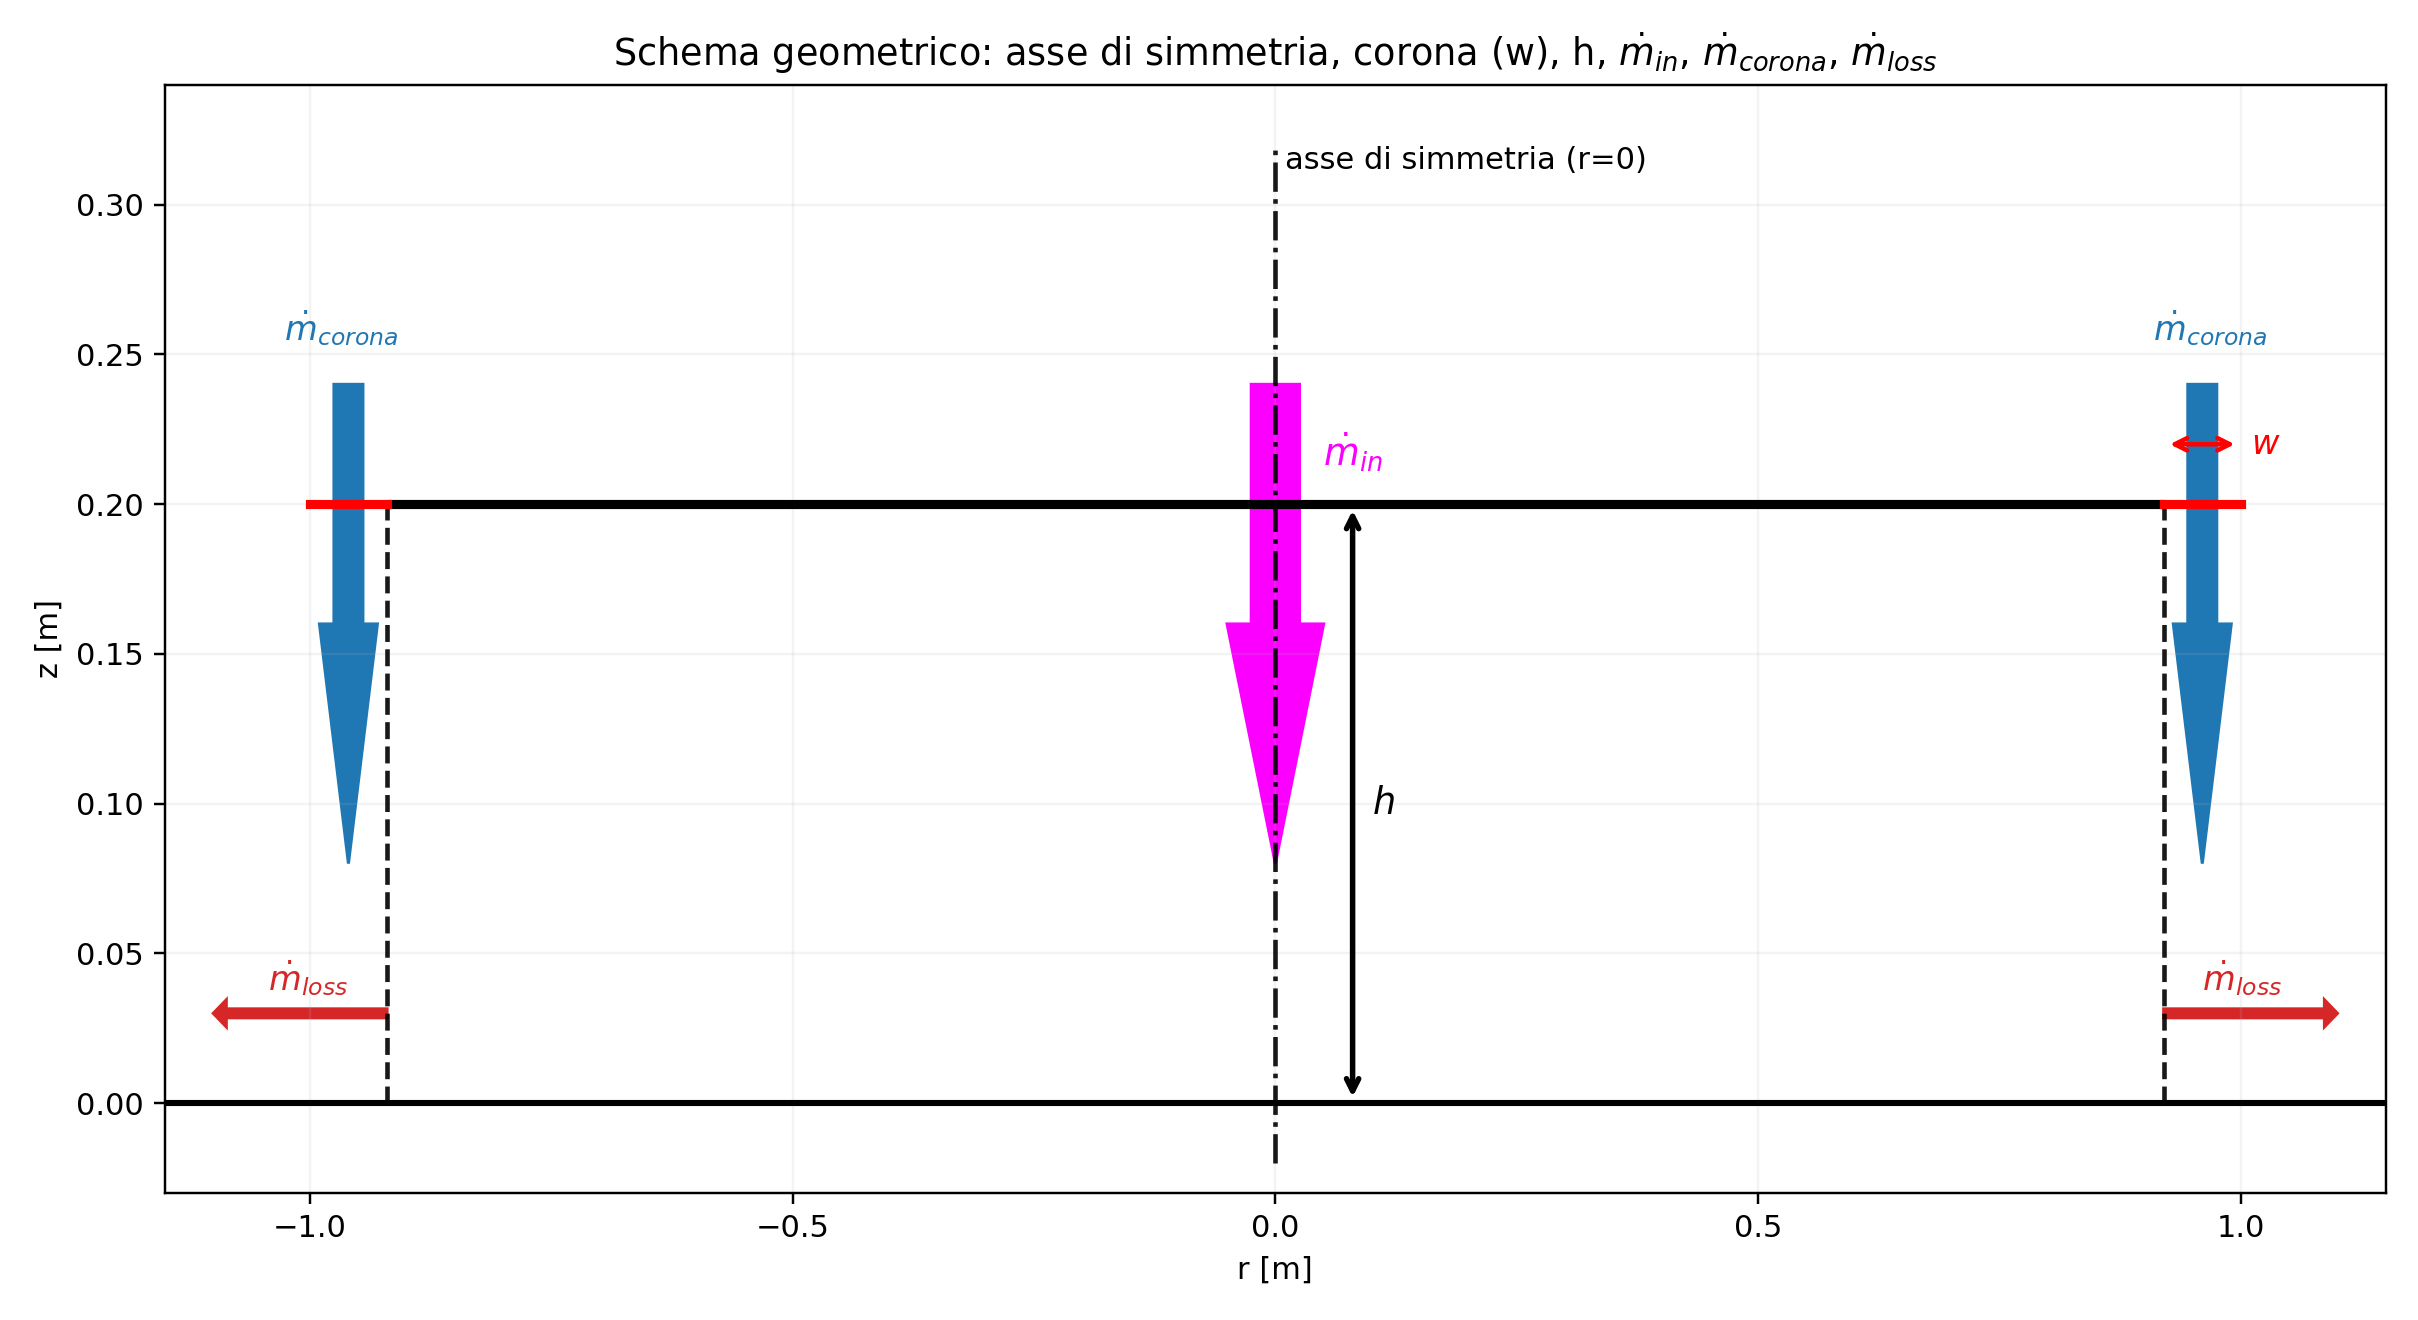
\includegraphics[width=0.95\linewidth]{../figs/schema_geometry.png}
  \caption{Geometry and notation. Figures produced by the Python script are saved under \texttt{../figs/}.}
  \label{fig:geometry}
\end{figure}

\section{Core Model (Design-Oriented)}
We use an anisotropic Stokes--Darcy closure for the mean core flow (low-Mach, no swirl):
\begin{equation}
  u = -\frac{\kappa_r}{\mu}\,\partial_r p,\qquad
  w = -\frac{\kappa_z}{\mu}\,\partial_z p,\qquad
  \kappa_r=\alpha_r h^2,\ \kappa_z=\alpha_z h^2,
  \label{eq:darcy}
\end{equation}
with compressible continuity
\begin{equation}
  \frac{1}{r}\,\partial_r\!\big(r\,\rho\,u\big)+\partial_z(\rho\,w)=0,\qquad
  p=\rho R_g T.
  \label{eq:cont_state}
\end{equation}
Eliminating $(u,w)$ yields the elliptic pressure problem on the core domain $r\in[0,R^-]$, $z\in[0,h]$:
\begin{equation}
  \frac{1}{r}\,\partial_r\!\big(r\,\rho\,\kappa_r\,\partial_r p\big)+\partial_z\!\big(\rho\,\kappa_z\,\partial_z p\big)=0,
  \label{eq:elliptic_dim}
\end{equation}
with boundary conditions: symmetry at $r=0$ ($\partial_r p=0$), no-normal-flow at $z=0$ and $z=h$ ($\partial_z p=0$ for the Darcy closure), and sealing pressure at the rim $r=R^-$,
\begin{equation}
  p_\mathrm{edge}(z)=p_0 + \Delta p\,\Phi\!\left(\frac{z}{h}\right),
  \qquad \Delta p = C_t\,\frac{\rho_j U_\mathrm{corona}^2\,b}{h_\mathrm{eff}},
  \label{eq:rim_bc}
\end{equation}
with a prescribed vertical distribution $\Phi(\zeta)$ (e.g.\ increasing in $\zeta$ to enforce downward core flow, $w<0$).

\section{Non-Dimensionalization}
Define dimensionless coordinates and fields
\begin{equation}
  \hat r=\frac{r}{R_{\text{tot}}},\quad
  \hat z=\frac{z}{h},\quad
  \hat p=\frac{p-p_0}{p_c},\quad
  \hat T=\frac{T}{T_\infty},
  \label{eq:nondim_vars}
\end{equation}
and $\rho_\infty=p_0/(R_g T_\infty)$, so
\begin{equation}
  \hat\rho=\frac{\rho}{\rho_\infty}=\frac{1+\Pi_p\,\hat p}{\hat T},\qquad
  \Pi_p=\frac{p_c}{p_0}.
  \label{eq:rho_hat}
\end{equation}
Introduce the anisotropy and geometry parameters
\begin{equation}
  \mathcal{A}=\frac{\kappa_z/h^2}{\kappa_r/R_{\text{tot}}^2}
  =\frac{\alpha_z}{\alpha_r}\left(\frac{R_{\text{tot}}}{h}\right)^2,\qquad
  \hat R^-=\frac{R^-}{R_{\text{tot}}}.
  \label{eq:A_param}
\end{equation}
Then the non-dimensional elliptic equation is
\begin{equation}
  \boxed{\
  \frac{1}{\hat r}\,\partial_{\hat r}\!\Big(\hat r\,\hat\rho\,\partial_{\hat r}\hat p\Big)
  + \mathcal{A}\,\partial_{\hat z}\!\Big(\hat\rho\,\partial_{\hat z}\hat p\Big)=0,\quad
  (\hat r,\hat z)\in[0,\hat R^-]\times[0,1].\ }
  \label{eq:elliptic_hat}
\end{equation}
Boundary conditions:
\begin{equation}
  \partial_{\hat r}\hat p(0,\hat z)=0,\quad
  \partial_{\hat z}\hat p(\hat r,0)=\partial_{\hat z}\hat p(\hat r,1)=0,\quad
  \hat p(\hat R^-,\hat z)=\hat p_\mathrm{edge}(\hat z)=\Pi_\mathrm{edge}\,\Phi(\hat z),
  \label{eq:BC_hat}
\end{equation}
with the dimensionless rim amplitude
\begin{equation}
  \Pi_\mathrm{edge}=\frac{p_\mathrm{edge}-p_0}{p_c}
  =\frac{C_t\,\rho_j U_\mathrm{corona}^2\,b}{h_\mathrm{eff}\,p_c}.
  \label{eq:Pi_edge}
\end{equation}

\paragraph{Non-dimensional velocities and plotting.}
Natural velocity scales from \eqref{eq:darcy} are
\begin{equation}
  U_r^0=\frac{\kappa_r}{\mu}\,\frac{p_c}{R_{\text{tot}}},\qquad
  U_z^0=\frac{\kappa_z}{\mu}\,\frac{p_c}{h},\qquad
  S=\frac{U_z^0}{U_r^0}=\frac{\alpha_z}{\alpha_r}\,\frac{R_{\text{tot}}}{h}.
  \label{eq:U_scales}
\end{equation}
Define
\begin{equation}
  \hat u=-\partial_{\hat r}\hat p,\qquad
  \hat w=-\partial_{\hat z}\hat p.
  \label{eq:vel_hat}
\end{equation}
For quiver with isotropic scaling in the plot plane, use vectors $(\hat u,\,S\,\hat w)$.
Report colormaps of $\hat p$, $|\hat u|$, $|\hat w|$, and optionally
\begin{equation}
  \hat V_{\mathrm{iso}}=\sqrt{\hat u^{\,2}+S^{2}\hat w^{\,2}}.
\end{equation}
Axes must be labeled $\hat r\in[0,\hat R^-]$ and $\hat z\in[0,1]$; colorbars are non-dimensional.

\section{Simulation Outputs (from \texttt{../figs/})}
Once the Python script is updated to emit non-dimensional fields, figures should be saved under \texttt{../figs/} with labels indicating hatted quantities, e.g. \texttt{cmap\_p\_hat.png}, \texttt{cmap\_u\_hat.png}, \texttt{cmap\_w\_hat.png}, and a quiver using $(\hat u,S\hat w)$.
The vertical reference at $\hat r=\hat R^-$ should be drawn in every plot.
Existing dimensional figures can still be shown; the non-dimensional ones enable parameter-agnostic comparison across runs.

\end{document}
